%------------------------------------------------------------------------------------------------------------
\section{Data structures and fonctionality} \label{sec:DataStructures}
%------------------------------------------------------------------------------------------------------------

An overview of the data structures implemented in the AMIDST toolbox is illustrated in Figure \ref{Figure:ToolboxDataStructures}. These data structures basically define the main components that will be used for implementing the AMIDST learning and inference algorithms. As we previously mentioned, in the AMIDST toolbox, we focus on two specific instantiations of PGMs, namely, a static Bayesian network (\comp{BN} component) and a two time-slice dynamic Bayesian network (\comp{2T-DBN} component). This is also directly reflected in the component structure.

\vspace{-0.1in}

\begin{figure}[ht!]
\begin{center}
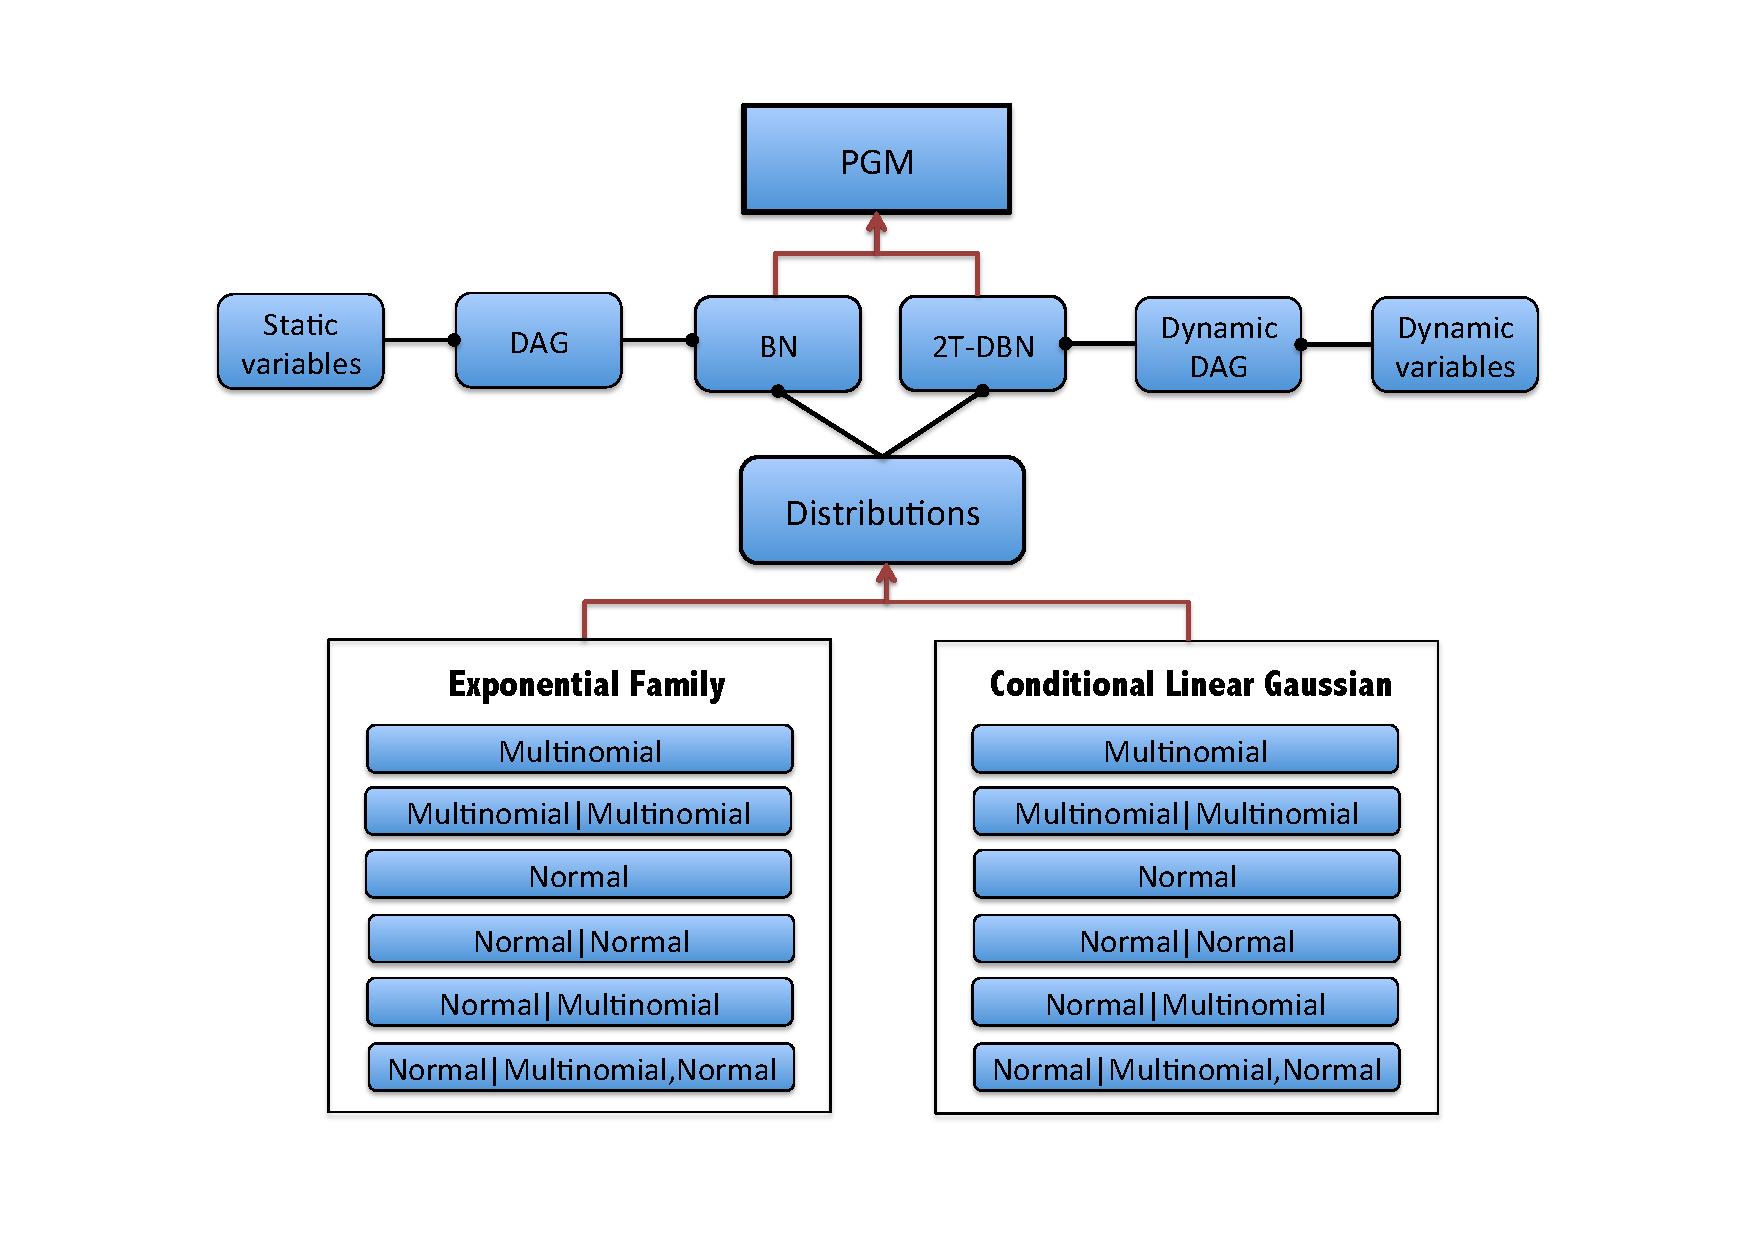
\includegraphics[width=\linewidth]{./figures/DataStructure}
\vspace{-0.5in}
\caption{\label{Figure:ToolboxDataStructures} Illustration of AMIDST toolbox data structure components. Nomenclature: The boxes in the
      figure represent software components (sets, possibly singletons, of classes), a rounded-arc going from $X$ to $Y$ indicates that $Y$ 'uses/references' $X$, and an arc with an arrow from $X$ to $Y$ implies inheritance.}
\end{center}
\end{figure}

In what follows, we briefly define each component and show how they can be used in the AMIDST toolbox through code excerpts. We describe first the components related to the static BN, i.e., \comp{Static variables}, \comp{DAG}, and \comp{BN}, then those related to the two time-slice dynamic BN, i.e., \comp{Dynamic variables}, \comp{Dynamic DAG}, and \comp{2T-DBN}. Finally, we present the \comp{Distributions} component that includes implementations of conditional probability distributions relying on two different representations, namely, \comp{Conditional Linear Gaussian} and \comp{Exponential Family} distributions. 

%------------------------------------------------------------------------------------------------------------
\subsection{Static variables}
%------------------------------------------------------------------------------------------------------------

Static variables consist of a list of objects of type Variable that are used later to build a static BN. Each static variable is characterized by its name, an ID, a state space type, and a distribution type (i.e., multinomial or normal). 

Note that static variables can be either initialised using the list of attributes that are parsed from a given data set or specified by the user. The following source code example shows how to define a set of five static variables:

\vspace{-0.1in}
\begin{table}[H]
\begin{tabular}{l} \\ \hline

        \texttt{StaticVariables variables = new StaticVariables(data.getAttributes());}\\

        \texttt{Variable A = variables.getVariableByName("A");}\\
        \texttt{Variable B = variables.getVariableByName("B");}\\
        \texttt{Variable C = variables.getVariableByName("C");}\\
        \texttt{Variable D = variables.getVariableByName("D");}\\

        \texttt{Variable H = variables.newMultionomialVariable("Hidden",}\\ \texttt{~~~~~~~~~~~~~~~~~~~~~~~~~Arrays.asList("TRUE", "FALSE"));}\\ \hline 

\end{tabular}
\end{table}


%------------------------------------------------------------------------------------------------------------
\subsection{Directed acyclic graph (\comp{DAG})}
%------------------------------------------------------------------------------------------------------------

A directed acyclic graph (\comp{DAG}) defines the BN graphical structure over a list of \comp{static variables}, such that the dependence relationships between the variables are established through the definition of the parent set for each variable. 

The following source code example shows how to build a \comp{DAG} over the previously defined set of static variables. The hidden variable is set as a parent of all the remaining variables:

\vspace{-0.1in}
\begin{table}[H]
\begin{tabular}{l} \\ \hline

        \texttt{DAG dag = new DAG(variables);}\\\\

        \texttt{dag.getParentSet(A).addParent(H);}\\
        \texttt{dag.getParentSet(B).addParent(H);}\\
        \texttt{dag.getParentSet(C).addParent(H);}\\
        \texttt{dag.getParentSet(D).addParent(H);}\\\\
        
        \texttt{System.out.println(dag.toString());}\\\hline 

\end{tabular}
\end{table}

The last line converts the resulting \texttt{dag} into a String object, then prints it to the standard console. We obtain:

\vspace{-0.1in}
\begin{table}[H]
\small{\begin{tabular}{l} \\
\texttt{DAG}\\
\texttt{A parent sets: \{Hidden\}}\\
\texttt{B parent sets: \{Hidden\}}\\
\texttt{C parent sets: \{Hidden\}}\\
\texttt{D parent sets: \{Hidden\}}\\
\texttt{Hidden parent sets: \{\}}\\
\end{tabular}}
\end{table}

%------------------------------------------------------------------------------------------------------------
\subsection{Bayesian network (\comp{BN})}
%------------------------------------------------------------------------------------------------------------

As mentioned before, a static BN consists of two components: a graphical structure (defined by the \comp{DAG} component) and a conditional probability distribution for each variable given its parent set (defined by the \comp{Distributions} component). Thus, given a DAG, the BN is defined by initialising the distribution of each variable according to its type and the type of its parent set.

The following brief code fragment shows how to define a BN using a previously build \texttt{dag}. It automatically checks the distribution type of each variable and its corresponding parents to uniformly initialise the \comp{Distributions} objects such as multinomial, normal, CLG, etc. (see Section \ref{subsec:Distributions}).


\begin{table}[H]
\begin{tabular}{l} \hline  
        \texttt{BayesianNetwork bnet = BayesianNetwork.newBayesianNetwork(dag);}\\ 
        \texttt{System.out.println(bnet.toString());}\\ \hline 
\end{tabular}
\end{table}      

Similarly to \comp{DAG} objects, the resulting \texttt{bnet} can be converted into a String object and printed to the standard console:

\begin{table}[H]
\small{\begin{tabular}{l} \\
\texttt{Bayesian Network:}\\
\texttt{P(A|Hidden) follows a Multinomial|Multinomial}\\
\texttt{[ 0.5, 0.5 ]}\\
\texttt{[ 0.5, 0.5 ]}\\
\texttt{P(B|Hidden) follows a Multinomial|Multinomial}\\
\texttt{[ 0.5, 0.5 ]}\\
\texttt{[ 0.5, 0.5 ]}\\
\texttt{P(C|Hidden) follows a Normal|Multinomial}\\
\texttt{Normal [ mu = 0.0, sd = 1.0 ]}\\
\texttt{Normal [ mu = 0.0, sd = 1.0 ]}\\
\texttt{P(D|Hidden) follows a Normal|Multinomial}\\
\texttt{Normal [ mu = 0.0, sd = 1.0 ]}\\
\texttt{Normal [ mu = 0.0, sd = 1.0 ]}\\
\texttt{P(Hidden) follows a Multinomial}\\
\texttt{[ 0.5, 0.5 ]}\\

\end{tabular}}
\end{table}

\begin{table}[H]
\small{\begin{tabular}{l} \\

\texttt{\% The probabilities can be then modified as follows:}\\\\

\texttt{Multinomial\_MultinomialParents distA = bnet.getDistribution(A);}\\
\texttt{distA.getMultinomial(0).setProbabilities(new double[]\{0.7, 0.3\});}\\
\texttt{distA.getMultinomial(1).setProbabilities(new double[]\{0.2, 0.8\});}\\\\

\texttt{Normal\_MultinomialParents distC = bnet.getDistribution(C);}\\
\texttt{distC.getNormal(0).setMean(0.15);}\\
\texttt{distC.getNormal(0).setSd(0.5);}\\
\texttt{distC.getNormal(1).setMean(0.24);}\\
\texttt{distC.getNormal(1).setSd(1);}\\

\end{tabular}}
\end{table}

%------------------------------------------------------------------------------------------------------------
\subsection{Dynamic variables}
%------------------------------------------------------------------------------------------------------------

The dynamic variables in a \comp{2T-DBN} are represented by a list of objects named allVariables and temporalClones of type \texttt{Variable}. Each dynamic variable is characterized by its name, ID, a state space type, and a distribution type (i.e., multinomial or normal). 

In order to represent the variables in a previous time step (needed when defining the dynamic DAG), we use the concept of \textit{temporal clone} variables, which are copies of the real main variables but refer to the previous time step. For instance, $X^{t-1}$ is codified as the \textit{temporal clone} of variable $X^t$. Hence, in our data structures, the time index $t$ is not explicitly represented for a dynamic variable, but implicitly considered with the use of \textit{temporal clones}.

The list of dynamic variables is initialised using the list of Attributes that are parsed from a given data set or specified by the user. Next, temporal clones are created through invoking the \texttt{getTemporalClone()} method. The following source code example shows how to define a set of six dynamic variables and a single temporal clone:

\vspace{-0.1in}
\begin{table}[H]
\begin{tabular}{l} \\ \hline

        \texttt{DynamicVariables dynamicVariables = new DynamicVariables(data.getAttributes());}\\

        \texttt{Variable A = dynamicVariables.getVariable("A");}\\
        \texttt{Variable B = dynamicVariables.getVariable("B");}\\
        \texttt{Variable C = dynamicVariables.getVariable("C");}\\
        \texttt{Variable D = dynamicVariables.getVariable("D");}\\
        
        \texttt{Variable ATempClone = dynamicVariables.getTemporalClone(A);}\\

        \texttt{Variable H1 = dynamicVariables.newMultinomialDynamicVariable("Hidden1",}\\ \texttt{~~~~~~~~~~~~~~~~~~~~~~~~~Arrays.asList("TRUE", "FALSE"));}\\ 
         \texttt{Variable H2 = dynamicVariables.newMultinomialDynamicVariable("Hidden2",}\\ \texttt{~~~~~~~~~~~~~~~~~~~~~~~~~Arrays.asList("TRUE", "FALSE"));}\\ \hline
\end{tabular}
\end{table}

%------------------------------------------------------------------------------------------------------------
\subsection{Dynamic directed acyclic graph (\comp{Dynamic DAG})}
%------------------------------------------------------------------------------------------------------------

A dynamic directed acyclic graph (\comp{Dynamic DAG}) is defined over a list of \comp{dynamic variables}. This component specifies the graph structure of a \comp{2T-DBN} by specifying the parent set for each dynamic variable at time $0$ and time $T > 0$.

The following source code example shows how to build a \comp{dynamic DAG} over the previously defined set of dynamic variables. 

\vspace{-0.1in}
\begin{table}[H]
\begin{tabular}{l} \\ \hline

        \texttt{DynamicDAG dynamicDAG = new DynamicDAG(dynamicVariables);}\\\\

        \texttt{dynamicDAG.getParentSetTime0(B).addParent(H1);}\\
        \texttt{dynamicDAG.getParentSetTime0(C).addParent(H1);}\\
        \texttt{dynamicDAG.getParentSetTime0(D).addParent(H1);}\\
        \texttt{dynamicDAG.getParentSetTime0(B).addParent(H2);}\\
        \texttt{dynamicDAG.getParentSetTime0(C).addParent(H2);}\\
        \texttt{dynamicDAG.getParentSetTime0(D).addParent(H2);}\\\\

        \texttt{dynamicDAG.getParentSetTimeT(A).addParent(ATempClone);}\\
        \texttt{dynamicDAG.getParentSetTimeT(B).addParent(H1);}\\
        \texttt{dynamicDAG.getParentSetTimeT(B).addParent(H2);}\\
        \texttt{dynamicDAG.getParentSetTimeT(C).addParent(H1);}\\
        \texttt{dynamicDAG.getParentSetTimeT(D).addParent(H1);}\\
        \texttt{dynamicDAG.getParentSetTimeT(D).addParent(H2);}\\
        \texttt{dynamicDAG.getParentSetTimeT(H1).addParent(ATempClone);}\\
        \texttt{dynamicDAG.getParentSetTimeT(H2).addParent(ATempClone);}\\\\
        
        \texttt{System.out.println(dynamicDAG.toString());}\\\hline 

\end{tabular}
\end{table}

The last line converts the resulting \texttt{dynamicDAG} into a String object, then prints it to the standard console:

\vspace{-0.1in}
\begin{table}[H]
\small{\begin{tabular}{l} \\

\texttt{Dynamic DAG at Time $0$}\\
\texttt{A has 0 parent(s): \{\}}\\
\texttt{B has 2 parent(s): \{Hidden1, Hidden2\}}\\
\texttt{C has 2 parent(s): \{Hidden1, Hidden2\}}\\
\texttt{D has 2 parent(s): \{Hidden1, Hidden2\}}\\
\texttt{Hidden1 has 0 parent(s): \{\}}\\
\texttt{Hidden2 has 0 parent(s): \{\}}\\\\

\texttt{Dynamic DAG at Time $T$}\\
\texttt{A has 1 parent(s): \{ATempClone\}}\\
\texttt{B has 2 parent(s): \{Hidden1, Hidden2\}}\\
\texttt{C has 2 parent(s): \{Hidden1, Hidden2\}}\\
\texttt{D has 2 parent(s): \{Hidden1, Hidden2\}}\\
\texttt{Hidden1 has 1 parent(s): \{ATempClone\}}\\
\texttt{Hidden2 has 1 parent(s): \{ATempClone\}}\\

\end{tabular}}
\end{table}

%------------------------------------------------------------------------------------------------------------
\subsection{Two time-slice dynamic Bayesian network (\comp{2T-DBN})}
%------------------------------------------------------------------------------------------------------------

Similarly to a static BN, a \comp{2T-DBN} (see Deliverable D2.1, Section 3.4 \cite{Deliverable2.1}) is defined using two main components: a graphical structure (defined by the \comp{Dynamic DAG} component) and a conditional probability distribution for each dynamic variable given its parent set (defined by the \comp{Distributions} component). Thus, given a \comp{Dynamic DAG}, the BN is defined by initialising the distributions of each dynamic variable at both time $0$ and time $T$ according to its type and the type of its parent set. 

This is brief code fragment showing the definition of a dynamic Bayesian network using the previously created \texttt{dynamicDAG}. It automatically looks at the distribution type of each variable and their parents to initialise the Distributions objects that are stored inside (i.e., Multinomial, Normal, CLG, etc). The parameters defining these distributions are correspondingly initialised.

The following brief code fragment shows how to define a \comp{2T-DBN} using a previously build \texttt{dynamicDAG}. It automatically checks the distribution type of each variable and its corresponding parents to uniformly initialise the \comp{Distribution} objects as multinomial, normal, CLG, etc. (see Section \ref{subsec:Distributions}).


\begin{table}[H]
\begin{tabular}{l} \hline  
        \texttt{DynamicBayesianNetwork dynamicbnet =}\\ \texttt{~~~~~~DynamicBayesianNetwork.newDynamicBayesianNetwork(dynamicDAG);}\\ 
        \texttt{System.out.println(dynamicbnet.toString());}\\ \hline 
\end{tabular}
\end{table}      


Similarly to \comp{dynamicDAG} objects, the resulting \texttt{dynamicbnet} can be converted into a String object and printed to the standard console:

\vspace{-0.1in}
\begin{table}[H]
\small{\begin{tabular}{l} \\

\texttt{Dynamic Bayesian Network Time 0:}\\
\texttt{P(A) follows a Multinomial}\\
\texttt{[ 0.5, 0.5 ]}\\
\texttt{P(B|Hidden1, Hidden2) follows a Multinomial|Multinomial}\\
\texttt{[ 0.5, 0.5 ]}\\
\texttt{[ 0.5, 0.5 ]}\\
\texttt{[ 0.5, 0.5 ]}\\
\texttt{[ 0.5, 0.5 ]}\\
\texttt{P(C|Hidden1, Hidden2) follows a Normal|Multinomial}\\
\texttt{Normal [ mu = 0.0, sd = 1.0 ]}\\
\texttt{Normal [ mu = 0.0, sd = 1.0 ]}\\
\texttt{Normal [ mu = 0.0, sd = 1.0 ]}\\
\texttt{Normal [ mu = 0.0, sd = 1.0 ]}\\

\texttt{P(D|Hidden1, Hidden2) follows a Normal|Multinomial}\\
\texttt{Normal [ mu = 0.0, sd = 1.0 ]}\\
\texttt{Normal [ mu = 0.0, sd = 1.0 ]}\\
\texttt{Normal [ mu = 0.0, sd = 1.0 ]}\\
\texttt{Normal [ mu = 0.0, sd = 1.0 ]}\\

\texttt{P(Hidden1) follows a Multinomial}\\
\texttt{[ 0.5, 0.5 ]}\\

\texttt{P(Hidden2) follows a Multinomial}\\
\texttt{[ 0.5, 0.5 ]}\\\\

\texttt{Dynamic Bayesian Network Time T:}\\
\texttt{P(A|ATempClone) follows a Multinomial|Multinomial}\\
\texttt{[ 0.5, 0.5 ]}\\
\texttt{[ 0.5, 0.5 ]}\\
\texttt{P(B|Hidden1, Hidden2) follows a Multinomial|Multinomial}\\
\texttt{[ 0.5, 0.5 ]}\\
\texttt{[ 0.5, 0.5 ]}\\
\texttt{[ 0.5, 0.5 ]}\\
\texttt{[ 0.5, 0.5 ]}\\
\texttt{P(C|Hidden1, Hidden2) follows a Normal|Multinomial}\\
\texttt{Normal [ mu = 0.0, sd = 1.0 ]}\\
\texttt{Normal [ mu = 0.0, sd = 1.0 ]}\\
\texttt{Normal [ mu = 0.0, sd = 1.0 ]}\\
\texttt{Normal [ mu = 0.0, sd = 1.0 ]}\\

\texttt{P(D|Hidden1, Hidden2) follows a Normal|Multinomial}\\
\texttt{Normal [ mu = 0.0, sd = 1.0 ]}\\
\texttt{Normal [ mu = 0.0, sd = 1.0 ]}\\
\texttt{Normal [ mu = 0.0, sd = 1.0 ]}\\
\texttt{Normal [ mu = 0.0, sd = 1.0 ]}\\

\texttt{P(Hidden1|ATempClone) follows a Multinomial|Multinomial}\\
\texttt{[ 0.5, 0.5 ]}\\
\texttt{[ 0.5, 0.5 ]}\\
\texttt{P(Hidden2|ATempClone) follows a Multinomial|Multinomial}\\
\texttt{[ 0.5, 0.5 ]}\\
\texttt{[ 0.5, 0.5 ]}\\

\end{tabular}}
\end{table}


%------------------------------------------------------------------------------------------------------------
\subsection{Distributions} \label{subsec:Distributions}
%------------------------------------------------------------------------------------------------------------

The \comp{Distributions} component consists of the set of conditional probability distributions considered in the AMIDST toolbox. It currently includes multinomial, normal, Dirichlet, and gamma distributions, and can easily be extended in the future to cover additional distribution types.

Note here that, in spite of the distinction between \comp{BN} and \comp{2T-BN}, the distributions over both models can be defined in the same way. In particular, the \comp{Distributions} component includes the set of conditional probability distributions considered in the AMIDST toolbox (the so-called \comp{Conditional Linear Gaussian} distributions, as detailed in Deliverable 2.1 \cite{Deliverable2.1}). More precisely, both variables with multinomial and normal distributions are modeled, and the distribution of each variable, in either a \comp{BN} or \comp{2T-BN}, is initialized and specified according to its distribution type and the distribution types of its potential parents. This consequently gives rise to the following different implemented probability distributions:

\begin{itemize}
  \item \comp{Multinomial}: a multinomial variable with no parents.
  \item \comp{Multinomial$|$Multinomial}: a multinomial variable with multinomial parents.
  \item \comp{Normal}: a normal variable with no parents.
  \item \comp{Normal$|$Normal}: a normal variable with normal parents.
  \item \comp{Normal$|$Multinomial}: a normal variable with multinomial parents.
  \item \comp{Normal$|$Multinomial,Normal}: a normal variable with a mixture of multinomial and normal parents.
\end{itemize}

The case of a multinomial variable having normal parents is not considered yet in this initial prototype. It is planned to be included in future versions, although strongly restricted in inference and learning algorithms due to the methodological and computational issues previously commented in Deliverable D2.1 \cite{Deliverable2.1}. 

We also provide an implementation of all the above distributions in the so-called \comp{Exponential Family} form, which ensures an alternative representation of the standard distributions based on vectors of natural and moment parameters. The implementation supports as well the Dirichlet and Gamma distributions for the \comp{Conjugate Priors} that will be used afterwards for learning.

The following brief code fragment shows the definition of the distribution for the discrete dynamic variable \texttt{A} at time $0$, and the continuous dynamic variable \texttt{C} given its two discrete parents at time $0$ too.

\begin{table}[H]
\begin{tabular}{l} \hline         
        \texttt{Multinomial distA = dynamicbnet.getDistributionTime0(A);}\\
        \texttt{distA.setProbabilities(new double[]\{0.1, 0.9\});}\\\\

        \texttt{Normal\_MultinomialParents distC = dynamicbnet.getDistributionTime0(C);}\\
        \texttt{distC.getNormal(0).setMean(0.7);}\\
        \texttt{distC.getNormal(0).setSd(0.2);}\\
        \texttt{distC.getNormal(1).setMean(0.4);}\\
        \texttt{distC.getNormal(1).setSd(1);}\\
        \texttt{distC.getNormal(2).setMean(0.75);}\\
        \texttt{distC.getNormal(2).setSd(0.05);}\\
        \texttt{distC.getNormal(3).setMean(0.66);}\\
        \texttt{distC.getNormal(3).setSd(0.04);}\\ \hline
\end{tabular}
\end{table}
